\section{Introduction}

\subsection{Motivation}
Traffic routing control aims at reducing congestion via providing drivers with route guidance. Nevertheless, it has been reported that driver non-compliance with routing instructions could undermine the performance of this management strategy \cite{powell2000value}, especially social routing advice that deliberately detours part of vehicles to achieve benefits in terms of road networks \cite{van2019travelers}. Besides, our previous paper showed in a theoretical manner that driver non-compliance could destabilize routed traffic systems  \cite{tang2023does}. 

Fortunately, it is promising to secure traffic routing control via pricing strategies. This is because monetary costs also play an important role in route choices \cite{kerkman2012car}. Indeed, applying joint routing and pricing polices is not a new idea \cite{yang1999evaluating}. However, to the best of our knowledge, few studies have conducted an analytical analysis of these management approaches, particularly considering stochastic driver compliance influenced by congestion and tolls.   

In this paper, we investigate the design of pricing policies that enhance driver adherence to route guidance, ensuring effective routing control. The major novelty lies in that we adopt a Markov chain to model drivers' compliance rates  conditioned on both traffic states and tolls. By formulating the managed traffic network as a nonlinear stochastic dynamical system, we can quantify in a more realistic way the impacts of driver route choices and thus determine appropriate tolls. Specially, we focus on a network comprised of two parallel links; see Figure~\ref{fig_twolink}. Though simple, the two-parallel-link network serves as a typical scenario for studying routing control; it turns out to be an appropriate abstraction of multiple parallel links: one stands for an arterial and the other denotes a set of local streets \cite{pi2017stochastic}. We assume that a reasonable routing policy is specified in advance, which means both the corridor $e_1$ and the local street $e_2$ are fully utilized if drivers completely obey the routing control. However, drivers could be reluctant to be detoured to link $e_2$. Thus a fixed toll $p$ is set on the corridor $e_1$ to give drivers incentives to choose the local street.

\begin{figure}[htbp]
    \centering
    \begin{subfigure}{0.4\linewidth}
        \centering
        \begin{tikzpicture}
        %Vertex
        \Vertex[x=0, style=black, size=0.1]{B}
        \Vertex[x=4, style=black, size=0.1]{N}
        %Edge
        \Edge[Direct,bend=30,lw=2pt](B)(N)
        \Edge[Direct,bend=330, lw=1pt](B)(N)
        \Edge[Direct,bend=315, lw=1pt](B)(N)
        \Edge[Direct,bend=300, lw=1pt](B)(N)
        \Text[x=2,y=0.9, fontsize=\footnotesize]{Corridor}
        \Text[x=2,y=-1.3, fontsize=\footnotesize]{Local streets}

        %Text
        \Text[x=-0.5,y=-0.4, fontsize=\footnotesize]{Origin}
        \Text[x=4.8,y=-0.4, fontsize=\footnotesize]{Destination}
    \end{tikzpicture}
    \caption{A network consisting of one corridor and multiple local streets.}
    \end{subfigure}
    \begin{subfigure}{0.4\linewidth}
        \centering
        \begin{tikzpicture}
        %Vertex
        \Vertex[x=-2.5,style={color=white}]{A}
        \Vertex[x=0, style=black, size=0.1]{B}
        \Vertex[x=4, style=black, size=0.1]{N}
        %Edge
        \Edge[Direct](A)(B)
        \Edge[Direct,bend=30](B)(N)
        \Edge[Direct,bend=330](B)(N)

        \Text[x=-1.25,y=0.2, fontsize=\footnotesize]{buffer $e_0$}
        \Text[x=2,y=0.9, fontsize=\footnotesize]{Corridor  $e_1$ with a fixed toll $p$}
        \Text[x=2,y=-0.9, fontsize=\footnotesize]{Local street  $e_2$}

        \Text[x=2,y=0.9, fontsize=\footnotesize]{}
        \Text[x=2,y=-1.3, fontsize=\footnotesize]{}
    \end{tikzpicture}
    \caption{An abstract of networks consisting of parallel links.}
    \end{subfigure}

    \caption{Modeling parallel-link networks.}
    \label{fig_twolink}
\end{figure}

%As for evaluating the given routing and pricing policies, we develop two theorems that verify whether the network is stabilizing or destabilizing subject to driver non-compliance. Furthermore, we propose using these theorems to derive lower bounds

%we adopt a Markov chain to model the compliance rate that possibly depends on traffic states. It allows us to study stability and instability criteria that determine whether the network is destabilized by the random compliance rate. We also quantify the impacts of drivers' disobedience in terms of throughput, namely the maximum constant inflow under which the network can be stabilized.


\subsection{Our contributions}
We try to address two main questions:
\begin{enumerate}
    \item[(i)] How to determine whether the network can be stabilized by routing and pricing strategies, subject to driver non-compliance?
    
    \item[(ii)] How to find the optimal pricing strategy that maximizes the network throughput, given a routing policy?
\end{enumerate}


The first question aims to assess the effectiveness of the given routing and pricing policies, where instability signals inadequate traffic management. To address this, we derive a stability condition (Theorem~\ref{thm_2}) using the Foster-Lyapunov criterion \cite{meyn2012markov} and an instability condition (Theorem~\ref{thm_3}) based on the transience of Markov chains \cite{meyn2012markov}.


It should be pointed out that the exact throughput cannot be determined, even for a simple two-parallel-link network, due to the randomness of driver non-compliance. To address the second question, we suggest using the stability and instability conditions to establish lower and upper bounds on throughput. This allows us to select suitable tolls that maximize these bounds.